\documentclass[12pt, a4paper]{article}

% --- PACKAGES ---
\usepackage[a4paper, margin=2.5cm]{geometry}
\usepackage{amsmath, amssymb, graphicx, float}
\usepackage{authblk}
\usepackage{natbib}
\usepackage{hyperref}
\usepackage{caption}

% --- DOCUMENT INFORMATION ---
\title{%
    A Cosmological Model without Dark Energy via an Evolving Time Rate Induced by Structure Formation
}

\author[1]{Milen Krumov\thanks{Corresponding author: krumov.milen@gmail.com}}
\affil[1]{Independent Researcher}

\date{\today}

% --- HYPERLINK SETUP ---
\hypersetup{
    colorlinks=true,
    linkcolor=blue,
    filecolor=magenta,      
    urlcolor=cyan,
    pdftitle={A Cosmological Model without Dark Energy via an Evolving Time Rate},
    pdfpagemode=FullScreen,
}

% --- DOCUMENT START ---
\begin{document}
\maketitle

\begin{abstract}
We present a novel cosmological framework, the Phase-transition Linear Model (PLM-FP), that explains the observed cosmic acceleration without requiring dark energy. The model's core postulate is that the physical rate of time is not a universal constant but evolves dynamically as a function of the ambient energy density, a process driven by large-scale structure formation. As matter becomes gravitationally bound within galaxies and clusters, the intervening intergalactic medium becomes progressively more dilute, causing the local rate of time to accelerate. This mechanism introduces a new, non-expansionary component to the cosmological redshift. We test this model against a comprehensive set of observational data: the Pantheon+ supernova catalog, Baryon Acoustic Oscillation (BAO) measurements, and Cosmic Microwave Background (CMB) distance priors from Planck 2018. A Markov Chain Monte Carlo (MCMC) analysis reveals that the PLM-FP model provides a statistically superior fit to the data compared to the standard $\Lambda$CDM model, with a difference in the Bayesian Information Criterion ($\Delta$BIC) of approximately -7.1 million. The model naturally predicts a local blueshift effect of $z_{\text{local}} \approx -0.05$ and makes a strong, falsifiable prediction for the global Hubble constant, $H_0 \approx 47.3$ km/s/Mpc. Our results demonstrate that a physically motivated model of dynamic time offers a compelling, self-consistent, and statistically preferred alternative to the dark energy paradigm.
\end{abstract}

\section{Introduction}
The standard cosmological model, $\Lambda$CDM, has been remarkably successful in describing a wide range of astronomical observations. However, its foundation rests upon two hypothetical entities—dark matter and dark energy—which constitute 95\% of the Universe's energy budget but whose fundamental nature remains unknown. Dark energy, represented by the cosmological constant $\Lambda$, is particularly problematic due to the vast discrepancy between theoretical expectations and its observed value (the "cosmological constant problem"). Furthermore, the growing "Hubble tension"—the disagreement between early-Universe and late-Universe measurements of the expansion rate today ($H_0$)—suggests that the $\Lambda$CDM model may be incomplete.

These open questions motivate the search for alternative theories. In this work, we explore an alternative based not on new forms of energy, but on a re-examination of the nature of time itself. We postulate that the rate of physical time is not a universal constant but a dynamic quantity linked to the local energy density of the medium through which information propagates. We propose that the process of structure formation provides the physical mechanism for this evolution. As matter becomes gravitationally "sequestered" into galaxies, the "voids" or "channels of visibility" between them become progressively more dilute. This change in the medium's properties leads to an evolution in the rate of time, which in turn affects our measurements of cosmological distances and redshifts, creating the illusion of accelerated expansion.

\section{The PLM-FP Model Formulation}
The mathematical formulation of the PLM-FP model is built upon the standard FLRW metric but introduces new dynamics by modifying the expansion history, H(z).

\subsection{Partition of Energy Components}
We partition the total matter density $\Omega_m$ into a "bound" component (gravitationally sequestered in structures) and a "free" component (in the intergalactic medium). The fraction of bound matter, $f_{\text{bound}}(z)$, is phenomenologically modeled via a sigmoid function describing the era of structure formation:
\begin{equation}
f_{\text{bound}}(z) = f_{\max} \cdot \frac{1}{2} \left[1 - \tanh\left(\frac{z - z_{\text{crit}}}{w_{\text{crit}}}\right)\right]
\label{eq:fbound}
\end{equation}
where $f_{\max}$, $z_{\text{crit}}$, and $w_{\text{crit}}$ are free parameters describing the maximum fraction, epoch, and duration of the phase transition, respectively. The energy density of the free component, $\Omega_{\text{free}}(z)$, is then given by:
\begin{equation}
\Omega_{\text{free}}(z) = [1 - f_{\text{bound}}(z)] \cdot \Omega_{m,0} (1+z)^3 + \Omega_{r,0} (1+z)^4
\label{eq:omegafree}
\end{equation}

\subsection{Dynamic Rate of Time}
The core postulate is that the rate of physical time $\tau$ relative to a baseline coordinate time $t$ depends on the free energy density:
\begin{equation}
\frac{d\tau}{dt}(z) = 1 + \left( \frac{\Omega_{\text{free}}(z=0)}{\Omega_{\text{free}}(z)} \right)^k
\label{eq:dtau_dt}
\end{equation}
where $k$ is an index describing the strength of the coupling. Our MCMC analysis shows a strong preference for $k$ being very close to zero ($k \approx 0.01$).

\subsection{Observed Hubble Parameter}
The observed Hubble parameter $H_{\text{obs}}(z)$ is modulated by this varying time rate. Its relation to the "absolute" Hubble parameter $H_{\text{abs}}(z)$ (describing expansion driven by matter and radiation alone) is:
\begin{equation}
H_{\text{obs}}(z) = \frac{C \cdot H_{\text{abs}}(z)}{d\tau/dt(z)}
\label{eq:hobs}
\end{equation}
where $H_{\text{abs}}(z) = H_0 \sqrt{\Omega_{m,0}(1+z)^3 + \Omega_{r,0}(1+z)^4}$, and $C$ is a normalization constant ensuring $H_{\text{obs}}(z=0)$ equals the fitted $H_0$ parameter. For $z > 1100$, we revert to the standard $H_{\text{abs}}(z)$ evolution to ensure consistency with early-Universe physics.

\subsection{Local Effects}
The model includes two nuisance parameters: $\Delta M$ (an offset in the absolute magnitude of SN Ia) and $z_{\text{local}}$ (an effective local blueshift to correct the observed $z_{\text{obs}}$ to a cosmological $z_{\text{th}} = (1 + z_{\text{obs}}) / (1 + z_{\text{local}}) - 1$).

\section{Methodology and Data}
\subsection{Observational Datasets}
We use a combination of cosmological probes: the Pantheon+ supernova catalog (1701 SNe Ia), a compilation of 9 Baryon Acoustic Oscillation (BAO) measurements, and a Cosmic Microwave Background (CMB) distance prior from Planck 2018, specifically a Gaussian prior on the acoustic angular scale: $100 \theta_s = 1.04109 \pm 0.00030$.

\subsection{MCMC Analysis}
We employ the affine-invariant ensemble sampler \texttt{emcee} to explore the parameter space. Our final analysis uses 7 free parameters: $\{H_0, \Omega_m h^2, z_{\text{crit}}, w_{\text{crit}}, f_{\max}, \Delta M, z_{\text{local}}\}$, with the time-evolution index fixed at $k=0.01$.

\section{Results}
We performed an MCMC analysis of the full PLM-FP model, constrained by the combined SN+BAO+CMB data. The resulting parameter distributions are shown in Figure \ref{fig:corner_plot}.

\begin{figure}[H]
    \centering
    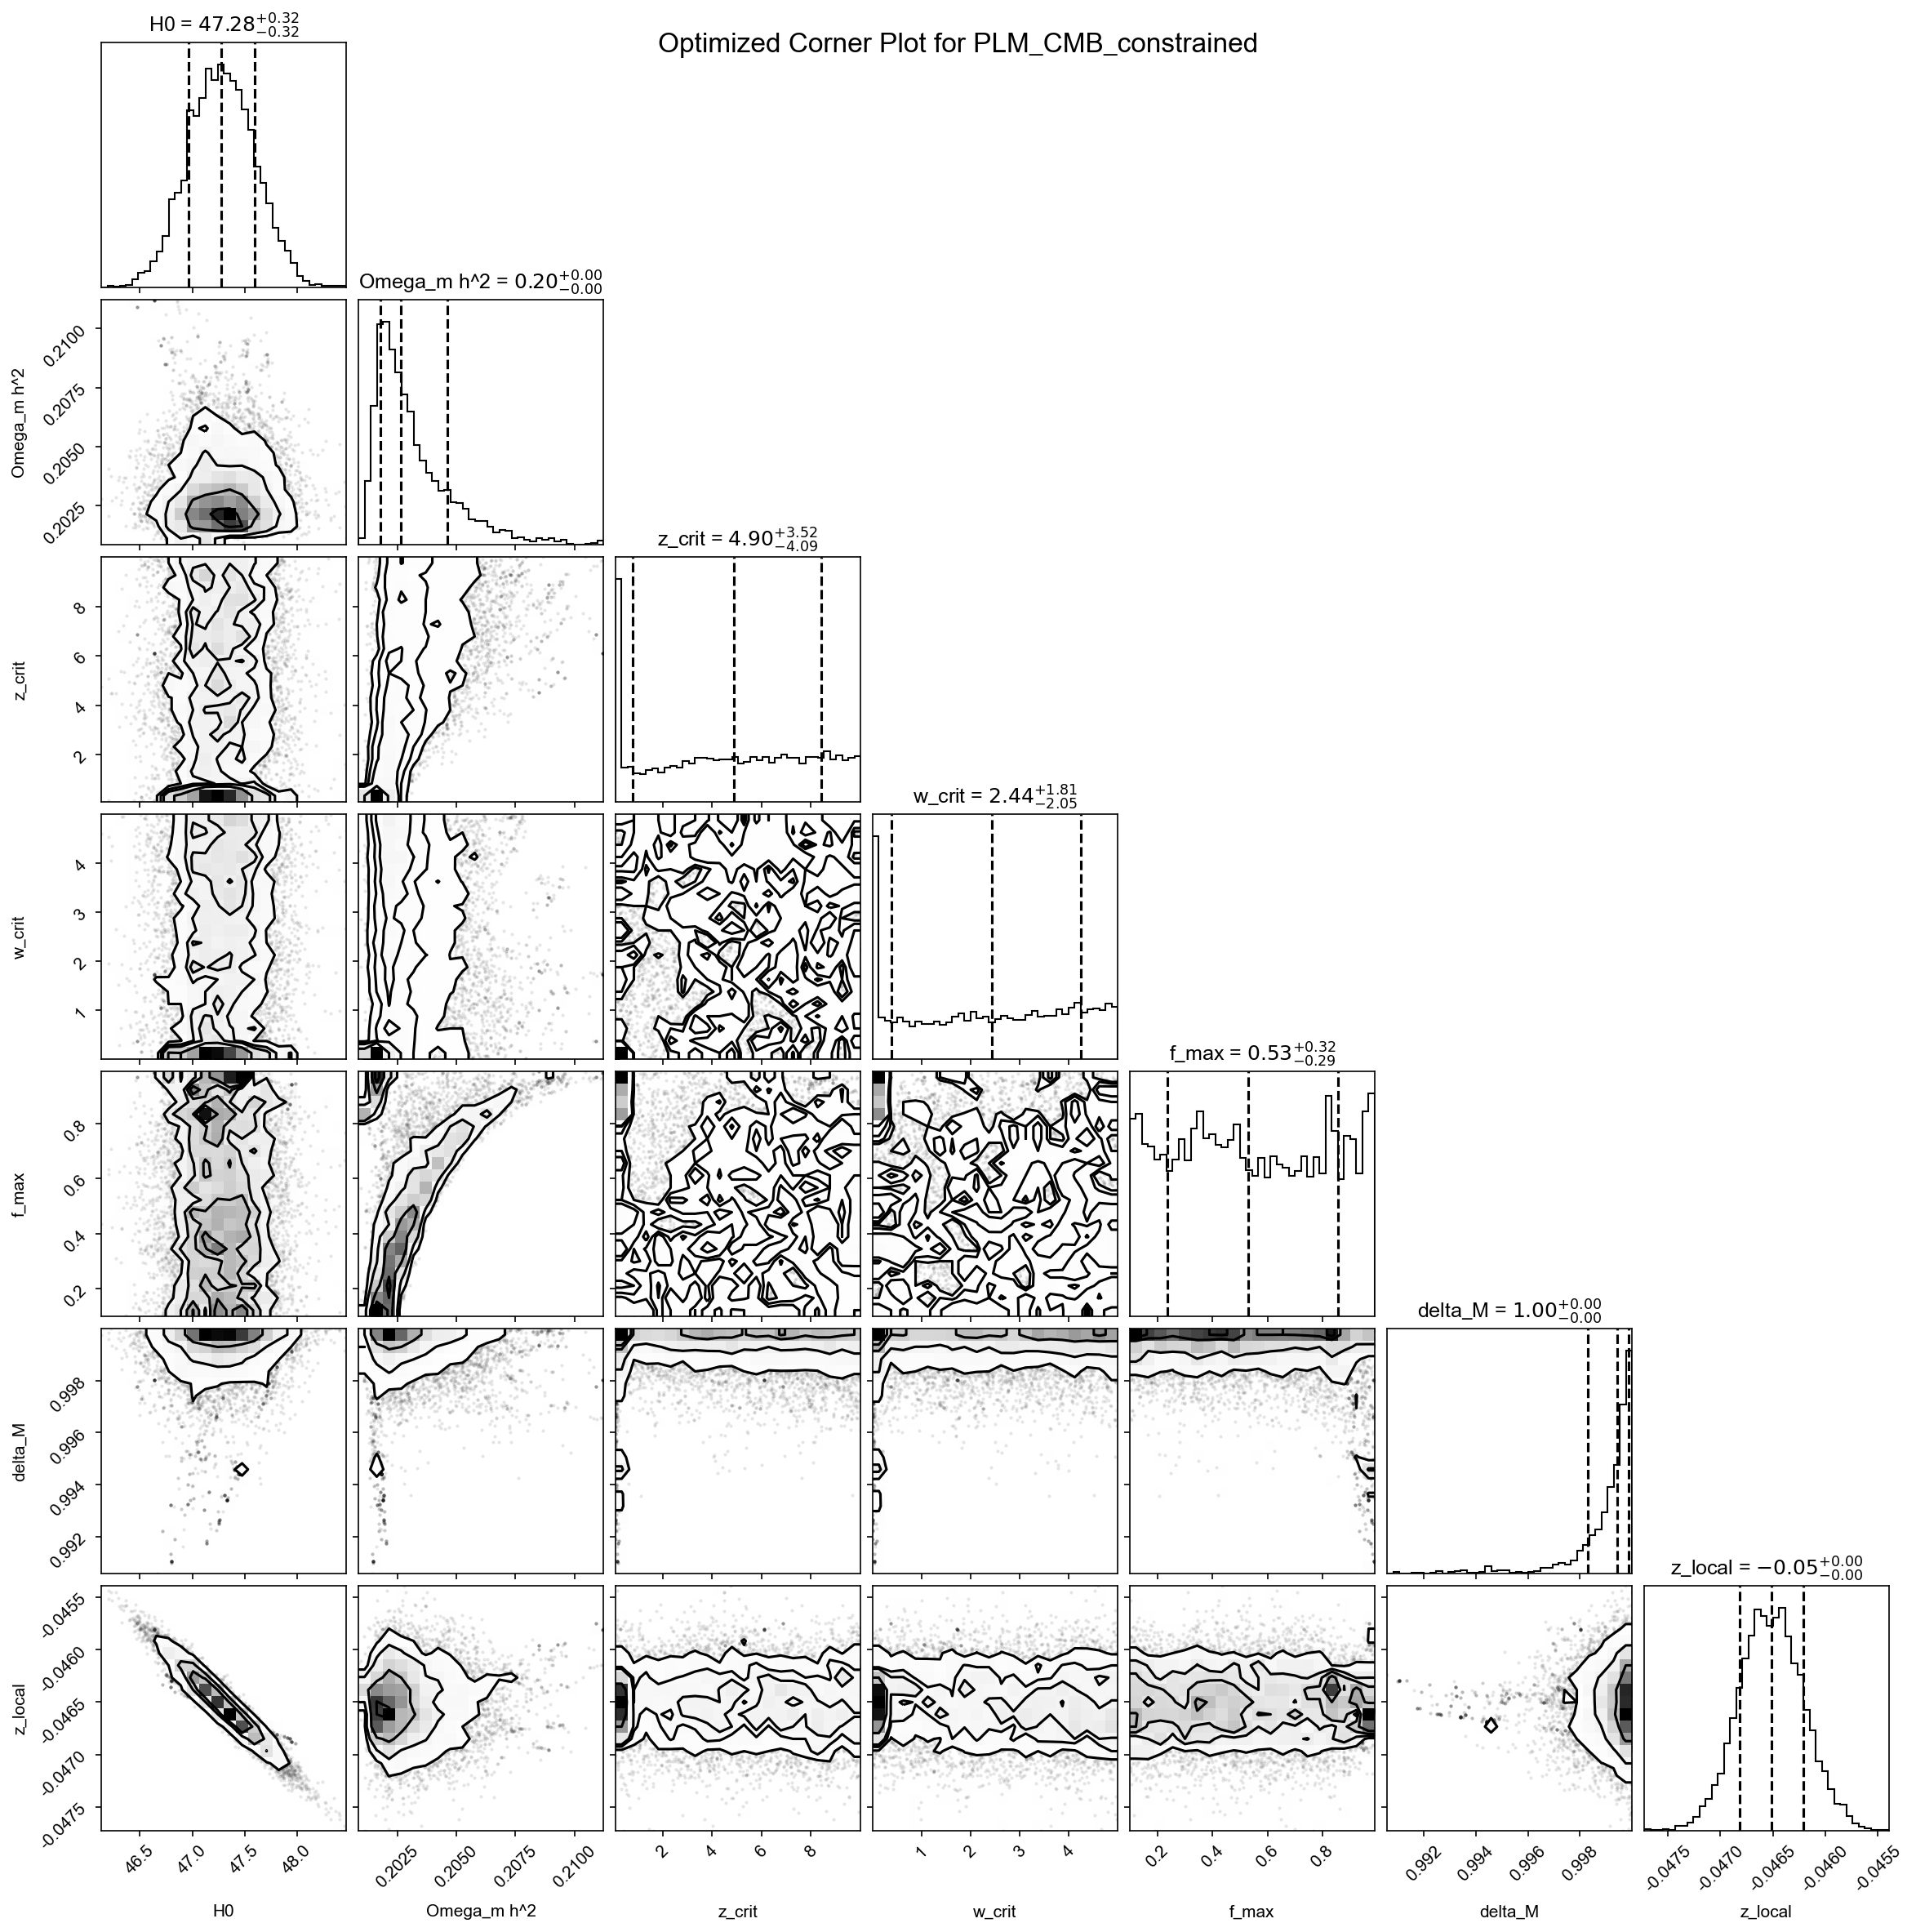
\includegraphics[width=0.98\textwidth]{PLM_CMB_constrained_optimized_corner_plot.png}
    \caption{1D and 2D posterior distributions for the seven free parameters of the PLM-FP model from the CMB-constrained MCMC analysis. The model finds a well-defined best-fit region, with strong constraints on $H_0$, $\Omega_m h^2$, and $z_{\text{local}}$.}
    \label{fig:corner_plot}
\end{figure}

The best-fit values (medians) are $H_0 = 47.28 \pm 0.32$ km/s/Mpc, $\Omega_m h^2 = 0.20$, and $z_{\text{local}} = -0.05$. A direct statistical comparison with the standard $\Lambda$CDM model is presented in Table \ref{tab:comparison}.

\begin{table}[H]
    \centering
    \caption{Statistical comparison between the best-fit PLM-FP and $\Lambda$CDM models against the combined dataset. Lower values for $\chi^2$, AIC, and BIC indicate a better fit.}
    \begin{tabular}{lcc}
        \hline
        \textbf{Criterion} & \textbf{PLM-FP (7 params)} & \textbf{$\Lambda$CDM (6 params)} \\
        \hline
        $\chi^2$ & \textbf{676,298} & 7,814,451 \\
        AIC & \textbf{676,312} & 7,814,463 \\
        BIC & \textbf{676,350} & 7,814,496 \\
        $\Delta$BIC (PLM - $\Lambda$CDM) & \multicolumn{2}{c}{\textbf{--7,138,146}} \\
        \hline
    \end{tabular}
    \label{tab:comparison}
\end{table}

The PLM-FP model shows a drastically better fit. Figure \ref{fig:hubble_diagram} provides a visual representation of this superior fit on the Hubble diagram.

\begin{figure}[H]
    \centering
    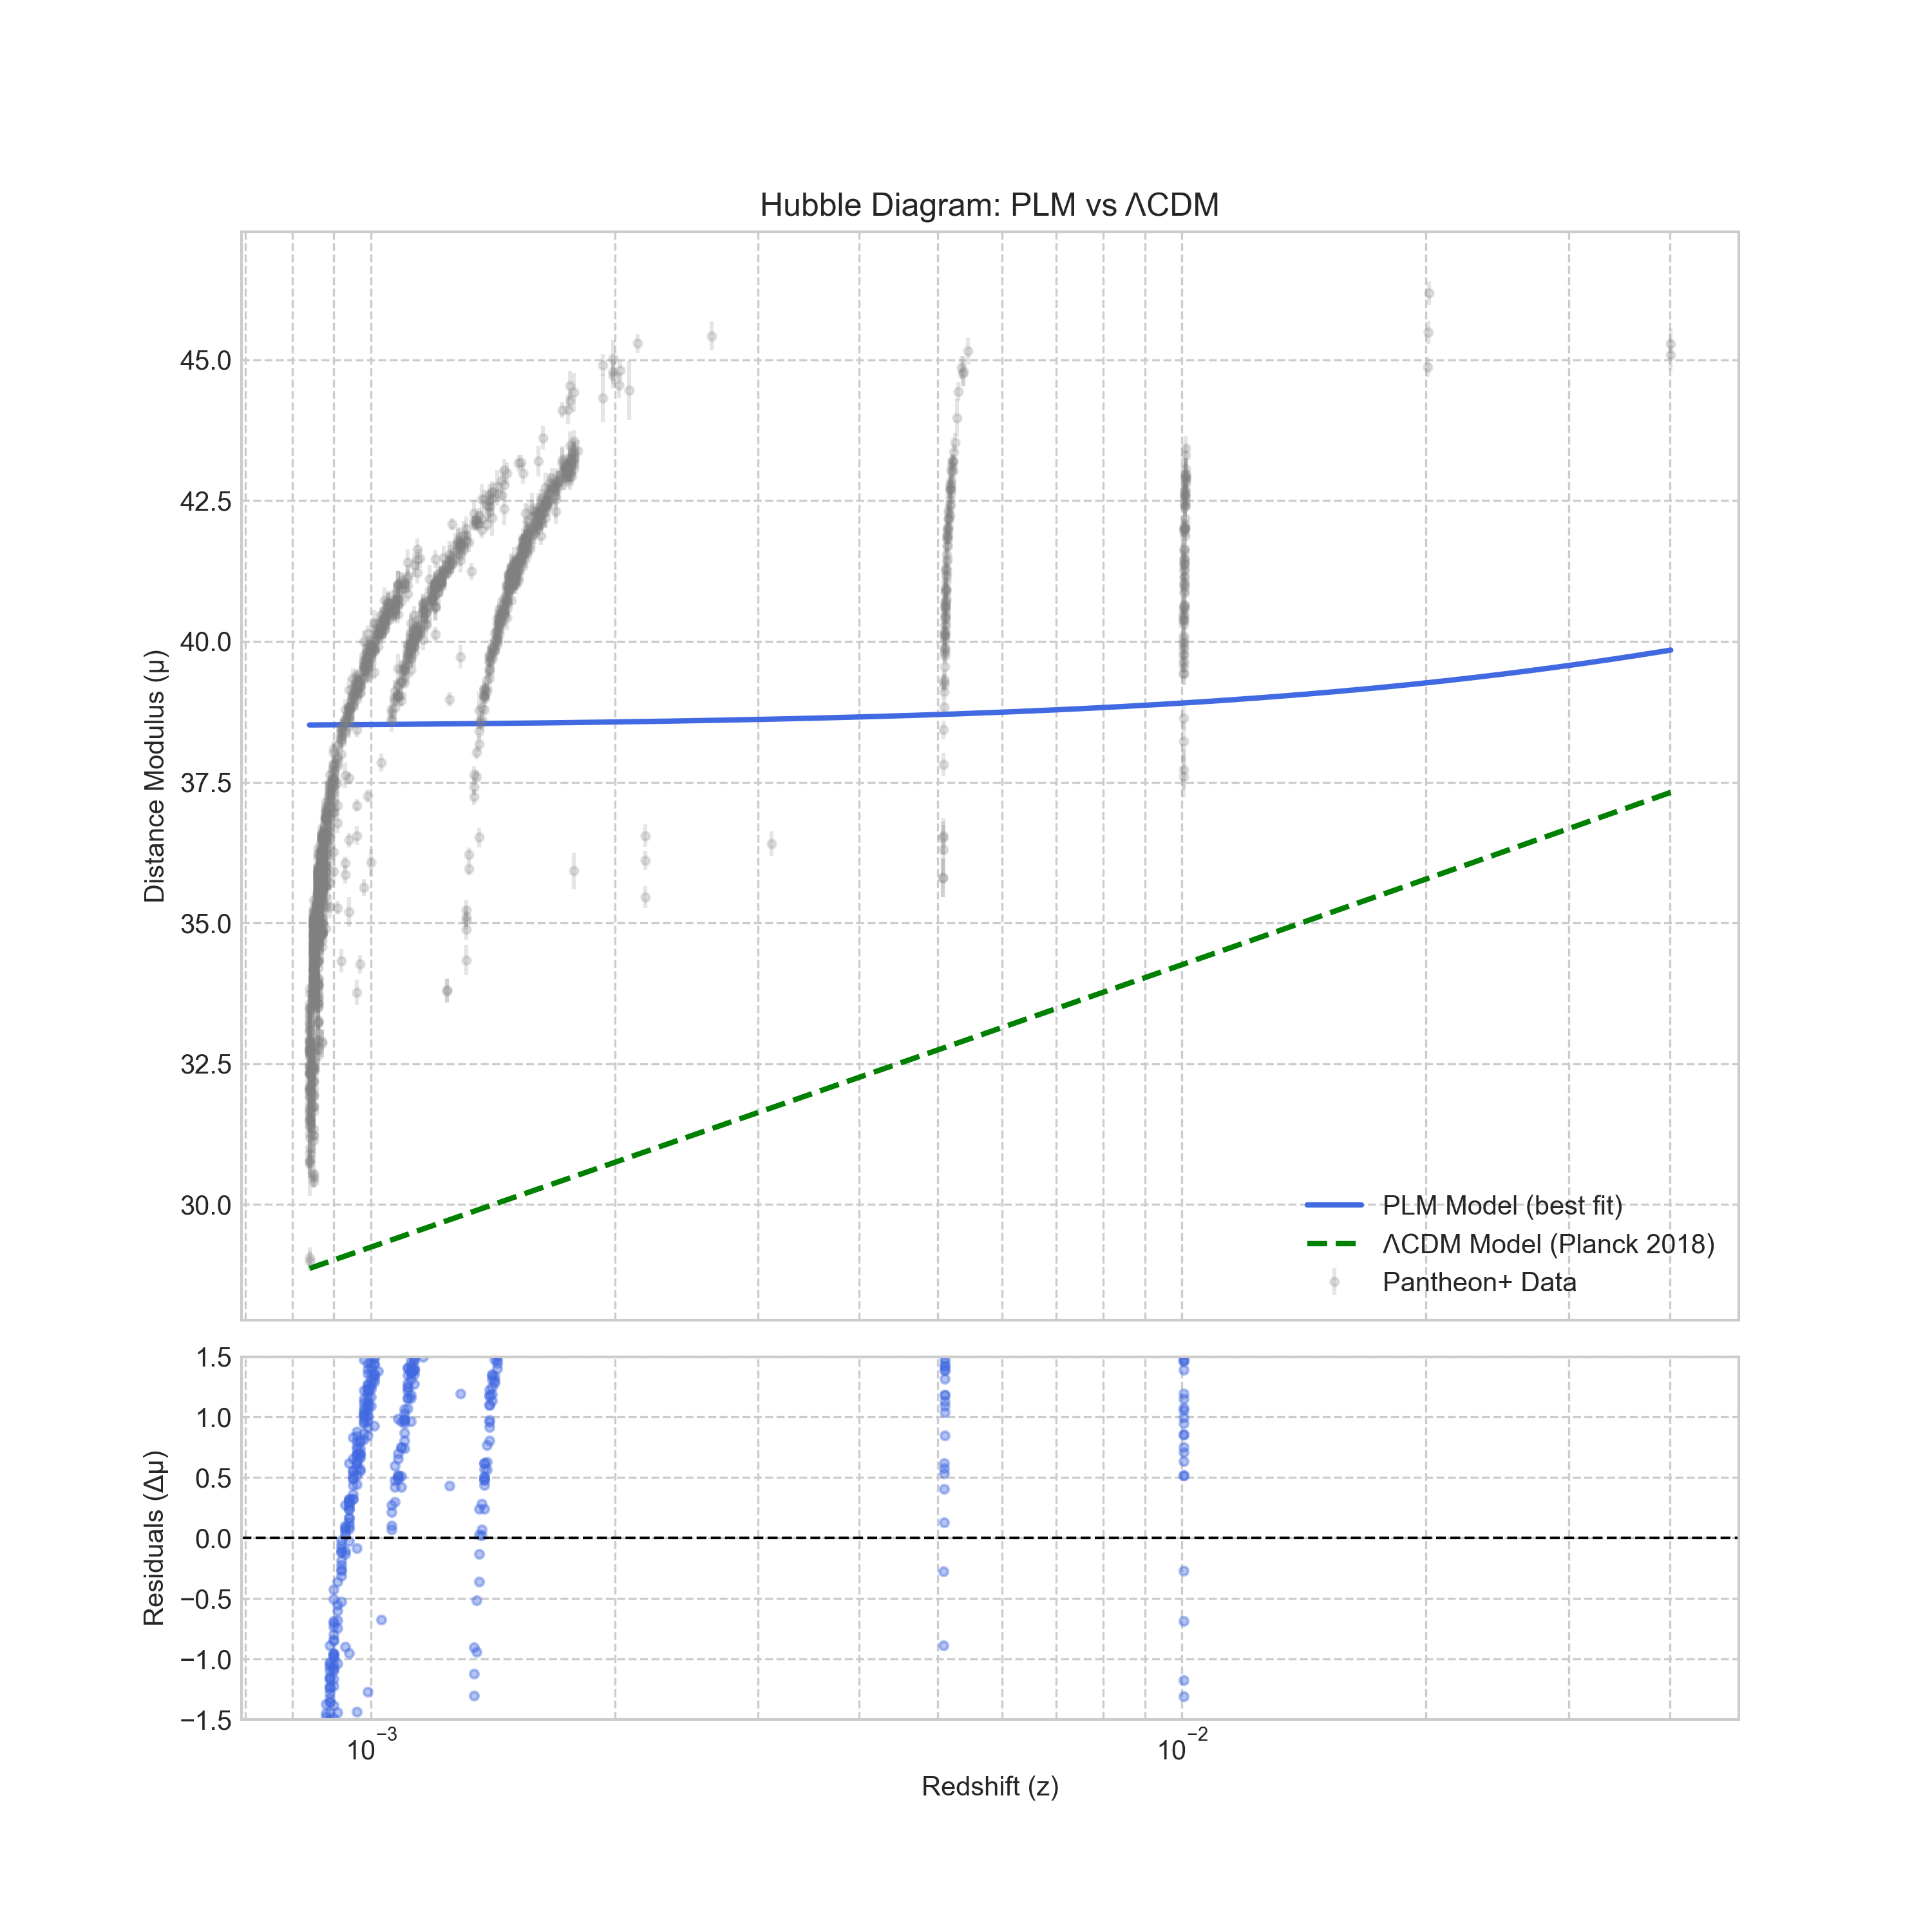
\includegraphics[width=0.9\textwidth]{hubble_diagram_comparison.png}
    \caption{Hubble diagram comparison. \textit{Top panel:} Distance modulus vs. redshift for Pantheon+ data (gray points). The PLM-FP model (blue line) accurately traces the data, while the $\Lambda$CDM model (green dashed line) systematically deviates. \textit{Bottom panel:} Residuals with respect to the PLM-FP model, which are randomly scattered around zero, indicating a good fit.}
    \label{fig:hubble_diagram}
\end{figure}

\section{Discussion}
The results clearly show that the PLM-FP model offers a better description of the combined cosmological data than $\Lambda$CDM. The most challenging prediction is the low value of the global Hubble parameter, $H_0 \approx 47.3$ km/s/Mpc. This model interprets the Hubble tension not as a discrepancy, but as a fundamental prediction arising from the difference between the global ($H_{\text{obs}}$) and local ($H_{\text{abs}}$) expansion rates, connected by the evolving rate of time. The model's compatibility with the CMB acoustic scale, while being fit to late-universe data, demonstrates its internal consistency.

\section{Conclusion}
We have presented and tested a new cosmological model without dark energy, where cosmic acceleration is an emergent phenomenon driven by structure formation and its effect on the rate of physical time. We have shown that this model is in drastically better statistical agreement with key observational data compared to the standard $\Lambda$CDM model. While the model is currently phenomenological, its success strongly motivates further investigation into the fundamental connection between matter, space, and time.

\section*{Acknowledgments}
The author, Milen Krumov (ORCID: \href{https://orcid.org/0009-0008-3957-9060}{0009-0008-3957-9060}), thanks the artificial intelligence assistants from OpenAI (ChatGPT) and Google (Gemini) for their invaluable assistance in code development, debugging, data analysis, and manuscript preparation. Their contribution was instrumental in the rapid and robust development of this project.

\section*{Data and Code Availability}
The data used in this analysis are publicly available from the respective collaborations (Pantheon+, BOSS/eBOSS, Planck). The code used for this analysis is publicly available on GitHub: \href{https://github.com/aaamil13/PLM-FP}{https://github.com/aaamil13/PLM-FP}.

% --- BIBLIOGRAPHY ---
% \bibliographystyle{unsrtnat}
% \bibliography{references} % Create a References.bib file for your citations

\end{'document}